\chapter{Introduction}
To all but the dinosaurs, meteors are quite cool.
\textcolor{red}{Broad idea of topic}
\section{Background}
Meteoroids are rocky or metallic bodies much smaller than asteroids, which, despite sizes ranging from a grain of sand to centimetres wide, produce streaks of light from the intense heat vaporising the meteoroid itself. At this point, it is a meteor. Meteoroids that survive the plummet to Earth are promoted meteorites. \\
The intense heat of a meteor ionises the air around it, causing the visible streak. This ionised air is capable of reflecting radio waves, allowing radio detection of meteors. The data that comes from detecting these ionised trails can be considered in various ways; most popularly by simply counting the number of detections an hour, or more visibly by displaying the intensity of the reflection for a range of frequencies across time. This produces a rather beautiful ``waterfall'' plot, as in figure \ref{fig:waterfall}.
My analysis focuses on six main areas of radio meteor detection; diurnal shift, zenithal hourly rate, shower detection, temporal \& spatial variation, mass, re-entry height \& line-of-sight velocity, and development of a meteor detection station. 
\begin{figure}[h!]
	\centering
	\begin{subfigure}{.24\textwidth}
		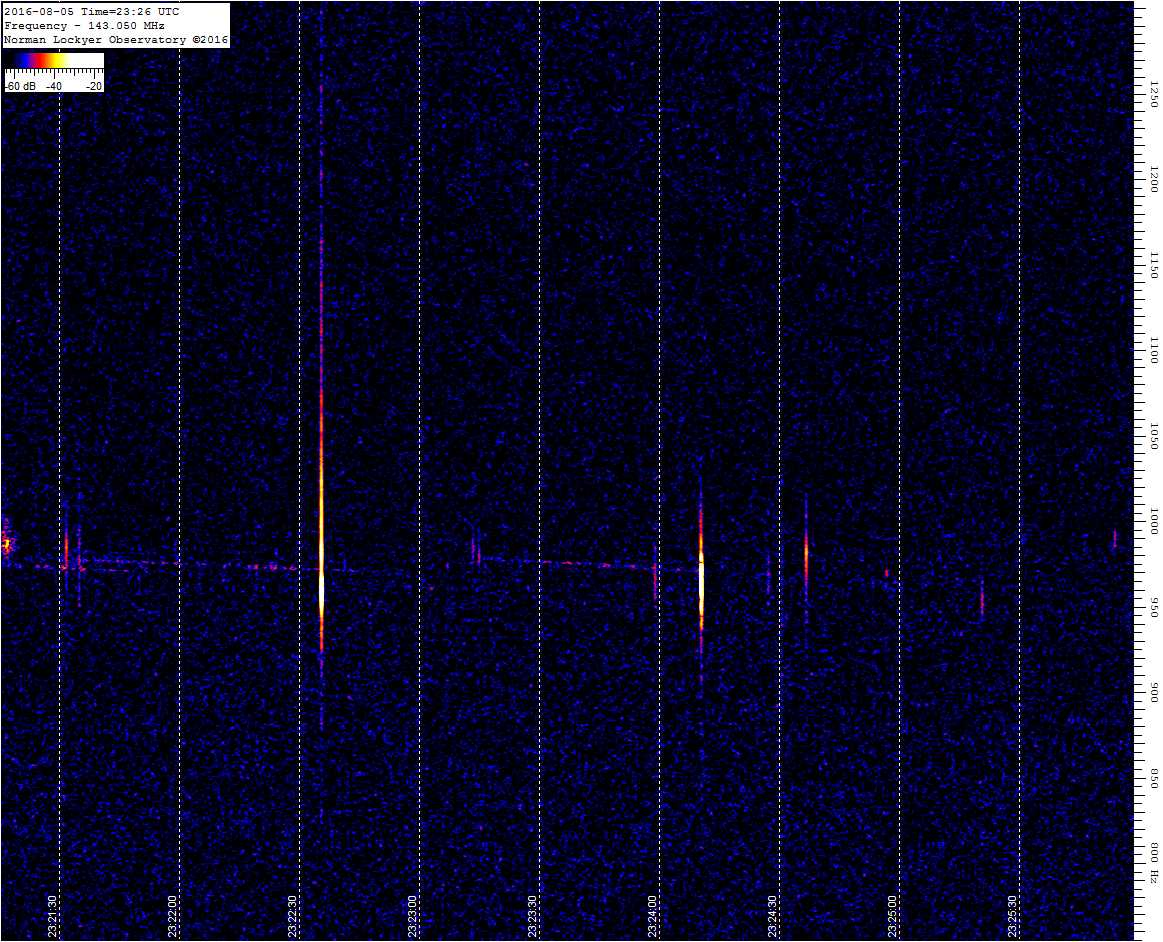
\includegraphics[width=\textwidth]{intro/2D}
		\caption{2D}
	\end{subfigure}
	\begin{subfigure}{.24\textwidth}
		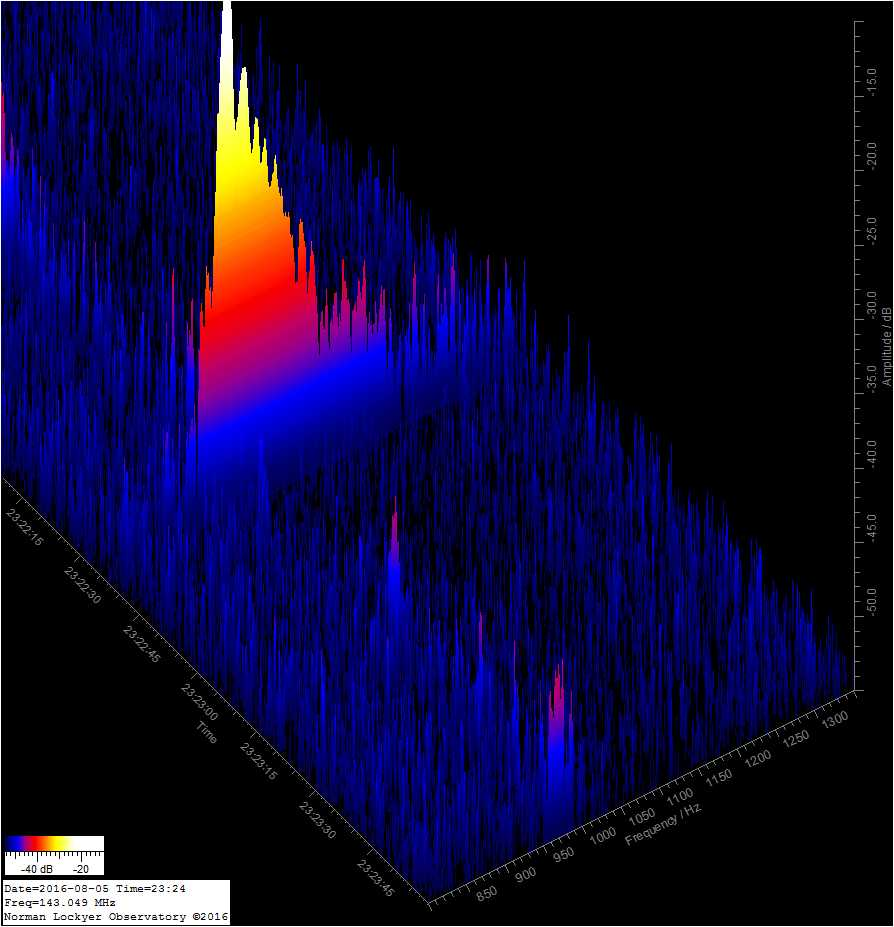
\includegraphics[width=\textwidth]{intro/3D}
		\caption{3D}
	\end{subfigure}
	\caption{Waterfall plot 
	\label{fig:waterfall}}
\end{figure}

Important things to explain: meteors, radiant, meteor shower, magnitude, meteor stream (for showers), 
